\documentclass{article}\usepackage[]{graphicx}\usepackage[]{color}
% maxwidth is the original width if it is less than linewidth
% otherwise use linewidth (to make sure the graphics do not exceed the margin)
\makeatletter
\def\maxwidth{ %
  \ifdim\Gin@nat@width>\linewidth
    \linewidth
  \else
    \Gin@nat@width
  \fi
}
\makeatother

\definecolor{fgcolor}{rgb}{0.345, 0.345, 0.345}
\newcommand{\hlnum}[1]{\textcolor[rgb]{0.686,0.059,0.569}{#1}}%
\newcommand{\hlstr}[1]{\textcolor[rgb]{0.192,0.494,0.8}{#1}}%
\newcommand{\hlcom}[1]{\textcolor[rgb]{0.678,0.584,0.686}{\textit{#1}}}%
\newcommand{\hlopt}[1]{\textcolor[rgb]{0,0,0}{#1}}%
\newcommand{\hlstd}[1]{\textcolor[rgb]{0.345,0.345,0.345}{#1}}%
\newcommand{\hlkwa}[1]{\textcolor[rgb]{0.161,0.373,0.58}{\textbf{#1}}}%
\newcommand{\hlkwb}[1]{\textcolor[rgb]{0.69,0.353,0.396}{#1}}%
\newcommand{\hlkwc}[1]{\textcolor[rgb]{0.333,0.667,0.333}{#1}}%
\newcommand{\hlkwd}[1]{\textcolor[rgb]{0.737,0.353,0.396}{\textbf{#1}}}%
\let\hlipl\hlkwb

\usepackage{framed}
\makeatletter
\newenvironment{kframe}{%
 \def\at@end@of@kframe{}%
 \ifinner\ifhmode%
  \def\at@end@of@kframe{\end{minipage}}%
  \begin{minipage}{\columnwidth}%
 \fi\fi%
 \def\FrameCommand##1{\hskip\@totalleftmargin \hskip-\fboxsep
 \colorbox{shadecolor}{##1}\hskip-\fboxsep
     % There is no \\@totalrightmargin, so:
     \hskip-\linewidth \hskip-\@totalleftmargin \hskip\columnwidth}%
 \MakeFramed {\advance\hsize-\width
   \@totalleftmargin\z@ \linewidth\hsize
   \@setminipage}}%
 {\par\unskip\endMakeFramed%
 \at@end@of@kframe}
\makeatother

\definecolor{shadecolor}{rgb}{.97, .97, .97}
\definecolor{messagecolor}{rgb}{0, 0, 0}
\definecolor{warningcolor}{rgb}{1, 0, 1}
\definecolor{errorcolor}{rgb}{1, 0, 0}
\newenvironment{knitrout}{}{} % an empty environment to be redefined in TeX

\usepackage{alltt}

\usepackage{float}

% Set the margins on the page to not be so large
\addtolength{\oddsidemargin}{-.875in}
\addtolength{\evensidemargin}{-.875in}
\addtolength{\textwidth}{1.75in}
\addtolength{\topmargin}{-.875in}
\addtolength{\textheight}{1.75in}

% Take off page numbering
\pagenumbering{gobble}
\IfFileExists{upquote.sty}{\usepackage{upquote}}{}
\begin{document}

\title{%
  4.1.1: R - Penalized Regression Methods \\
  (Ridge Regression, LASSO, and Elastic Net) \\
  \smallskip
  \large Stat 5100: Dr. Bean
}
\date{}

\maketitle

\subsubsection*{Matrix Specification}

Previously, when we have created linear models in this class, you have always seen the model be created in the form:

\begin{knitrout}
\definecolor{shadecolor}{rgb}{0.969, 0.969, 0.969}\color{fgcolor}\begin{kframe}
\begin{alltt}
\hlstd{linear_model} \hlkwb{<-} \hlkwd{lm}\hlstd{(response} \hlopt{~} \hlstd{x1} \hlopt{+} \hlstd{x2,} \hlkwc{data} \hlstd{= mydata)}
\end{alltt}
\end{kframe}
\end{knitrout}

However, when we create models in R, we don't always do it like this. Another way to specify models in R is with ``matrix specification.'' In matrix specification, instead of using the ``$\sim$'' syntax (this is called a formula in R), instead we pass in a matrix of the predictor variables and a vector of the response variable $y$. As an example:

\begin{knitrout}
\definecolor{shadecolor}{rgb}{0.969, 0.969, 0.969}\color{fgcolor}\begin{kframe}
\begin{alltt}
\hlcom{# Either:}
\hlstd{model} \hlkwb{<-} \hlkwd{somemodel}\hlstd{(y, X)}
\hlcom{# Or in some packages:}
\hlstd{model} \hlkwb{<-} \hlkwd{somemodel}\hlstd{(X, y)}
\end{alltt}
\end{kframe}
\end{knitrout}

In the above, the variable $X$ is a matrix in R where each column would contain our predictor variables $x_1$, $x_2$, etc. and our rows would contain the different observations. For example, $X_{i, j}$ (meaning the $i$th row of $X$ and the $j$th column of $X$) would refer to the recorded value of $x_j$ (the $j$th predictor variable for the the $i$th observation in our data.

The reason that this syntax is not always exactly synchronized with the formula notation you are used to, is because many model types in R are only available in community-created packages where it is up to the author to specify the form of their function's interface. The takeaway here is that when you learn how to use a new package, do not assume that everything will always be the same. Always look up a new package's documentation and learn how to use it.

In R, the most commonly used implementations of ridge regression and other penalized regression methods use matrix specification. It is important to keep in mind these implementations do not exist natively in R and are thus created by community users who later upload their package to CRAN (R's official repository). It is a good skill to learn how to use many types of functions as you will encounter many different types in your R career.

\medskip
\hrule
\medskip

\textbf{Example: } (Ridge Regression; recall Handout 2.6.1 example) A study seeks to relate (in females) amount of body fat ($Y$) to triceps skinfold thickness ($X_1$), thigh circumference ($X_2$), and midarm circumference ($X_3$).  Amount of body fat is expensive to measure, requiring immersion of person in water.  This expense motivates the desire for a predictive model based on these inexpensive predictors.

\begin{knitrout}
\definecolor{shadecolor}{rgb}{0.969, 0.969, 0.969}\color{fgcolor}\begin{kframe}
\begin{alltt}
\hlcom{# Load the data}
\hlkwd{library}\hlstd{(stat5100)}
\hlkwd{data}\hlstd{(bodyfat)}

\hlcom{# Look at the original fit along with VIF:}
\hlstd{bodyfat_lm} \hlkwb{<-} \hlkwd{lm}\hlstd{(body} \hlopt{~} \hlstd{triceps} \hlopt{+} \hlstd{thigh} \hlopt{+} \hlstd{midarm,} \hlkwc{data} \hlstd{= bodyfat)}

\hlkwd{summary}\hlstd{(bodyfat_lm)}
\end{alltt}
\begin{verbatim}
## 
## Call:
## lm(formula = body ~ triceps + thigh + midarm, data = bodyfat)
## 
## Residuals:
##     Min      1Q  Median      3Q     Max 
## -3.7263 -1.6111  0.3923  1.4656  4.1277 
## 
## Coefficients:
##             Estimate Std. Error t value Pr(>|t|)
## (Intercept)  117.085     99.782   1.173    0.258
## triceps        4.334      3.016   1.437    0.170
## thigh         -2.857      2.582  -1.106    0.285
## midarm        -2.186      1.595  -1.370    0.190
## 
## Residual standard error: 2.48 on 16 degrees of freedom
## Multiple R-squared:  0.8014,	Adjusted R-squared:  0.7641 
## F-statistic: 21.52 on 3 and 16 DF,  p-value: 7.343e-06
\end{verbatim}
\begin{alltt}
\hlcom{# VIF:}
\hlstd{olsrr}\hlopt{::}\hlkwd{ols_vif_tol}\hlstd{(bodyfat_lm)}
\end{alltt}
\begin{verbatim}
##   Variables   Tolerance      VIF
## 1   triceps 0.001410750 708.8429
## 2     thigh 0.001771971 564.3434
## 3    midarm 0.009559681 104.6060
\end{verbatim}
\begin{alltt}
\hlcom{# Try ridge regression as a remedial measure}
\hlcom{# -----------------------------------------}
\hlcom{# We use the glmnet() function inside the glmnet package to do this. Note that}
\hlcom{# instead of specifying our model using a formula (formulas in R are of the}
\hlcom{# form Y ~ X1 + X2 + X3), we create a dataframe of just our predictor variables}
\hlcom{# and a vector of our response variable.}
\hlstd{y} \hlkwb{<-} \hlstd{bodyfat}\hlopt{$}\hlstd{body}

\hlcom{# Our X must come in the form of a matrix. First we take out the "body" column}
\hlcom{# from the dataframe, and then we convert it to a matrix.}
\hlstd{X} \hlkwb{<-} \hlkwd{as.matrix}\hlstd{(}\hlkwd{subset}\hlstd{(bodyfat,} \hlkwc{select} \hlstd{=} \hlopt{-}\hlstd{body))}

\hlcom{# It is standard to standardize our variables in ridge regression. Note however}
\hlcom{# that if you forget to do this, you should be completely fine because}
\hlcom{# the implementations of ridge regression should standardize it for you}
\hlcom{# if you pass in an unstandardized X matrix.}
\hlstd{X} \hlkwb{<-} \hlkwd{scale}\hlstd{(X)}

\hlcom{# Select an optimal value for lambda. In glmnet, set alpha = 0 to do ridge regression.}
\hlcom{# This cv function here will selecte a value of lambda for you.}
\hlcom{# (Ignore the warning below)}
\hlstd{bodyfat_test_ridge_lm} \hlkwb{<-} \hlstd{glmnet}\hlopt{::}\hlkwd{cv.glmnet}\hlstd{(X, y,} \hlkwc{alpha} \hlstd{=} \hlnum{0}\hlstd{)}
\end{alltt}


{\ttfamily\noindent\color{warningcolor}{\#\# Warning: Option grouped=FALSE enforced in cv.glmnet, since < 3 observations per fold}}\begin{alltt}
\hlstd{bodyfat_test_ridge_lm}
\end{alltt}
\begin{verbatim}
## 
## Call:  glmnet::cv.glmnet(x = X, y = y, alpha = 0) 
## 
## Measure: Mean-Squared Error 
## 
##     Lambda Measure   SE Nonzero
## min  0.437   8.102 1.93       3
## 1se  4.473   9.882 2.07       3
\end{verbatim}
\end{kframe}
\end{knitrout}

Here let's pick $\lambda = 0.437$ based upon the above output.

\begin{knitrout}
\definecolor{shadecolor}{rgb}{0.969, 0.969, 0.969}\color{fgcolor}\begin{kframe}
\begin{alltt}
\hlcom{# Use the non-cv version to actually create a model that we can use and predict with.}
\hlstd{bodyfat_ridge_lm} \hlkwb{<-} \hlstd{glmnet}\hlopt{::}\hlkwd{glmnet}\hlstd{(X, y,} \hlkwc{alpha} \hlstd{=} \hlnum{0}\hlstd{,} \hlkwc{lambda} \hlstd{=} \hlnum{0.437}\hlstd{)}
\hlcom{# Looka at coefficients}
\hlstd{bodyfat_ridge_lm}\hlopt{$}\hlstd{beta}
\end{alltt}
\begin{verbatim}
## 3 x 1 sparse Matrix of class "dgCMatrix"
##                 s0
## triceps  2.1999416
## thigh    2.2873325
## midarm  -0.4351881
\end{verbatim}
\begin{alltt}
\hlcom{# Store our coefficients. You could do this by manually entering the numbers,}
\hlcom{# but I index them here for better automation.}
\hlstd{triceps_coef} \hlkwb{<-} \hlstd{bodyfat_ridge_lm}\hlopt{$}\hlstd{beta[}\hlnum{1}\hlstd{]}
\hlstd{thigh_coef} \hlkwb{<-} \hlstd{bodyfat_ridge_lm}\hlopt{$}\hlstd{beta[}\hlnum{2}\hlstd{]}
\hlstd{midarm_coef} \hlkwb{<-} \hlstd{bodyfat_ridge_lm}\hlopt{$}\hlstd{beta[}\hlnum{3}\hlstd{]}
\end{alltt}
\end{kframe}
\end{knitrout}

In order to get $b_0$ for the \textit{unstandardized} coefficients, we use the formula:
\[\beta_0 = \bar{Y} - \beta_1 \bar{X}_1 - \beta_2 \bar{X}_2 - \beta_3 \bar{X}_3\]

\begin{knitrout}
\definecolor{shadecolor}{rgb}{0.969, 0.969, 0.969}\color{fgcolor}\begin{kframe}
\begin{alltt}
\hlcom{# Means of various variables}
\hlkwd{mean}\hlstd{(bodyfat}\hlopt{$}\hlstd{body)}
\end{alltt}
\begin{verbatim}
## [1] 20.195
\end{verbatim}
\begin{alltt}
\hlkwd{mean}\hlstd{(bodyfat}\hlopt{$}\hlstd{triceps)}
\end{alltt}
\begin{verbatim}
## [1] 25.305
\end{verbatim}
\begin{alltt}
\hlkwd{mean}\hlstd{(bodyfat}\hlopt{$}\hlstd{thigh)}
\end{alltt}
\begin{verbatim}
## [1] 51.17
\end{verbatim}
\begin{alltt}
\hlkwd{mean}\hlstd{(bodyfat}\hlopt{$}\hlstd{midarm)}
\end{alltt}
\begin{verbatim}
## [1] 27.62
\end{verbatim}
\begin{alltt}
\hlcom{# Crunch our b0 formula:}
\hlstd{b0_estimate} \hlkwb{<-} \hlkwd{mean}\hlstd{(bodyfat}\hlopt{$}\hlstd{body)} \hlopt{-} \hlstd{(triceps_coef} \hlopt{*} \hlkwd{mean}\hlstd{(bodyfat}\hlopt{$}\hlstd{triceps))} \hlopt{-}
  \hlstd{(thigh_coef} \hlopt{*} \hlkwd{mean}\hlstd{(bodyfat}\hlopt{$}\hlstd{thigh))} \hlopt{-} \hlstd{(midarm_coef} \hlopt{*} \hlkwd{mean}\hlstd{(bodyfat}\hlopt{$}\hlstd{midarm))}
\hlstd{b0_estimate}
\end{alltt}
\begin{verbatim}
## [1] -140.4974
\end{verbatim}
\end{kframe}
\end{knitrout}

\subsubsection*{Get predicted values in ridge regression}

\begin{knitrout}
\definecolor{shadecolor}{rgb}{0.969, 0.969, 0.969}\color{fgcolor}\begin{kframe}
\begin{alltt}
\hlstd{predicted_y} \hlkwb{<-} \hlkwd{predict}\hlstd{(bodyfat_ridge_lm, X)}

\hlcom{# Plot the predicted values vs observed}
\hlkwd{plot}\hlstd{(y, predicted_y,} \hlkwc{xlab} \hlstd{=} \hlstr{"Observed Body Fat"}\hlstd{,} \hlkwc{ylab} \hlstd{=} \hlstr{"Predicted Body Fat"}\hlstd{,}
     \hlkwc{main} \hlstd{=} \hlstr{"Predicted Y vs. Observed Y in Ridge Regression"}\hlstd{)}
\end{alltt}
\end{kframe}

{\centering 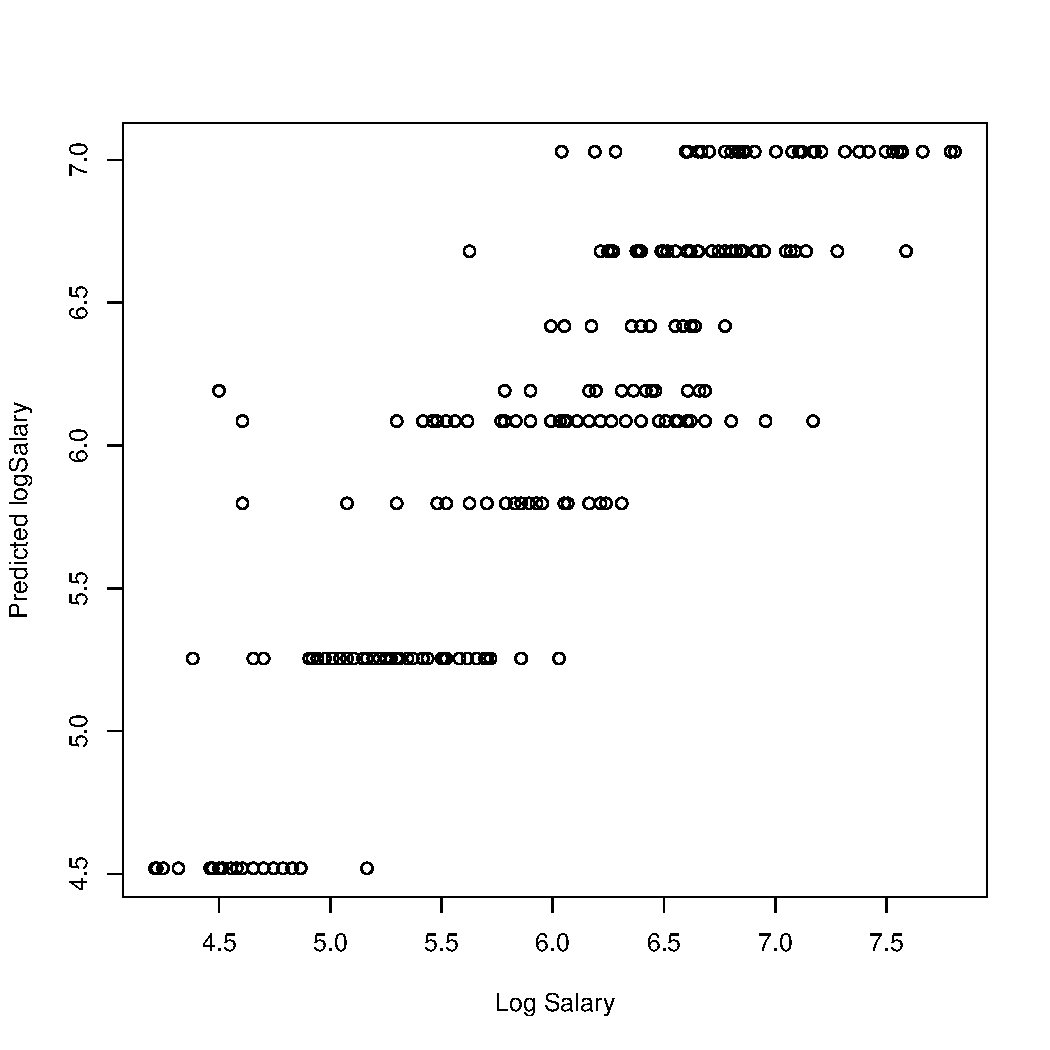
\includegraphics[width=0.6\textwidth]{figure/unnamed-chunk-6-1} 

}



\end{knitrout}

\medskip
\hrule
\medskip

\subsection*{Example 2: Baseball}

This data set (from SAS Help: the dataset has been imported into this R package) contains salary (for 1987) and performance (1986 and some career) data for 322 MLB players who played at least one game in both 1986 and 1987 seasons, excluding pitchers. How can salary be predicted from performance?

\begin{knitrout}
\definecolor{shadecolor}{rgb}{0.969, 0.969, 0.969}\color{fgcolor}\begin{kframe}
\begin{alltt}
\hlcom{# Load and take a look at the baseball dataset}
\hlkwd{data}\hlstd{(baseball)}
\hlkwd{head}\hlstd{(baseball)}
\end{alltt}
\begin{verbatim}
##                Name      Team nAtBat nHits nHome nRuns nRBI nBB YrMajor CrAtBat
## 1    Allanson, Andy Cleveland    293    66     1    30   29  14       1     293
## 2       Ashby, Alan   Houston    315    81     7    24   38  39      14    3449
## 3       Davis, Alan   Seattle    479   130    18    66   72  76       3    1624
## 4     Dawson, Andre  Montreal    496   141    20    65   78  37      11    5628
## 5 Galarraga, Andres  Montreal    321    87    10    39   42  30       2     396
## 6  Griffin, Alfredo   Oakland    594   169     4    74   51  35      11    4408
##   CrHits CrHome CrRuns CrRbi CrBB   League Division Position nOuts nAssts
## 1     66      1     30    29   14 American     East        C   446     33
## 2    835     69    321   414  375 National     West        C   632     43
## 3    457     63    224   266  263 American     West       1B   880     82
## 4   1575    225    828   838  354 National     East       RF   200     11
## 5    101     12     48    46   33 National     East       1B   805     40
## 6   1133     19    501   336  194 American     West       SS   282    421
##   nError Salary Div logSalary
## 1     20     NA  AE        NA
## 2     10  475.0  NW  6.163315
## 3     14  480.0  AW  6.173786
## 4      3  500.0  NE  6.214608
## 5      4   91.5  NE  4.516339
## 6     25  750.0  AW  6.620073
\end{verbatim}
\begin{alltt}
\hlcom{# First, we need to remove all NAs otherwise the algorithm will not work.}
\hlstd{baseball} \hlkwb{<-} \hlkwd{na.omit}\hlstd{(baseball)}

\hlcom{# Fit all this into matrix specification}
\hlstd{X_baseball} \hlkwb{<-} \hlkwd{as.matrix}\hlstd{(}\hlkwd{subset}\hlstd{(baseball,}
                               \hlkwc{select} \hlstd{=} \hlkwd{c}\hlstd{(nAtBat, nHits, nHome, nRuns, nRBI,}
                                          \hlstd{nBB, YrMajor, CrAtBat, CrHits, CrHome,}
                                          \hlstd{CrRuns, CrRbi, CrBB, nOuts, nAssts, nError)))}
\hlstd{y_baseball} \hlkwb{<-} \hlstd{baseball}\hlopt{$}\hlstd{logSalary}
\end{alltt}
\end{kframe}
\end{knitrout}

First, let's use Lasso regression:

\begin{knitrout}
\definecolor{shadecolor}{rgb}{0.969, 0.969, 0.969}\color{fgcolor}\begin{kframe}
\begin{alltt}
\hlstd{baseball_lasso_optimal} \hlkwb{<-} \hlstd{glmnet}\hlopt{::}\hlkwd{cv.glmnet}\hlstd{(X_baseball, y_baseball,} \hlkwc{alpha} \hlstd{=} \hlnum{1}\hlstd{)}
\hlstd{baseball_lasso_optimal}
\end{alltt}
\begin{verbatim}
## 
## Call:  glmnet::cv.glmnet(x = X_baseball, y = y_baseball, alpha = 1) 
## 
## Measure: Mean-Squared Error 
## 
##      Lambda Measure      SE Nonzero
## min 0.01390  0.3508 0.02621       8
## 1se 0.09805  0.3734 0.02771       7
\end{verbatim}
\begin{alltt}
\hlcom{# Pick optimal lambda from the above}
\hlstd{baseball_lasso} \hlkwb{<-} \hlstd{glmnet}\hlopt{::}\hlkwd{glmnet}\hlstd{(X_baseball, y_baseball,}
                                 \hlkwc{alpha} \hlstd{=} \hlnum{1}\hlstd{,} \hlkwc{lambda} \hlstd{= baseball_lasso_optimal}\hlopt{$}\hlstd{lambda.min)}
\hlstd{baseball_lasso}\hlopt{$}\hlstd{beta}
\end{alltt}
\begin{verbatim}
## 16 x 1 sparse Matrix of class "dgCMatrix"
##                    s0
## nAtBat   .           
## nHits    6.823840e-03
## nHome    1.638456e-03
## nRuns    .           
## nRBI     5.689562e-05
## nBB      5.994047e-03
## YrMajor  6.571314e-02
## CrAtBat  .           
## CrHits   2.571496e-04
## CrHome   .           
## CrRuns   .           
## CrRbi    .           
## CrBB     .           
## nOuts    1.830800e-04
## nAssts   .           
## nError  -6.013340e-03
\end{verbatim}
\end{kframe}
\end{knitrout}

Now, let's show an example with elastic net regression. Here we will pick $\alpha = 0.5$.

\begin{knitrout}
\definecolor{shadecolor}{rgb}{0.969, 0.969, 0.969}\color{fgcolor}\begin{kframe}
\begin{alltt}
\hlstd{baseball_elnet_optimal} \hlkwb{<-} \hlstd{glmnet}\hlopt{::}\hlkwd{cv.glmnet}\hlstd{(X_baseball, y_baseball,} \hlkwc{alpha} \hlstd{=} \hlnum{0.5}\hlstd{)}
\hlstd{baseball_elnet_optimal}
\end{alltt}
\begin{verbatim}
## 
## Call:  glmnet::cv.glmnet(x = X_baseball, y = y_baseball, alpha = 0.5) 
## 
## Measure: Mean-Squared Error 
## 
##      Lambda Measure      SE Nonzero
## min 0.02308  0.3536 0.03368      11
## 1se 0.21522  0.3822 0.03269       9
\end{verbatim}
\begin{alltt}
\hlcom{# Pick optimal lambda from the above}
\hlstd{baseball_elnet} \hlkwb{<-} \hlstd{glmnet}\hlopt{::}\hlkwd{glmnet}\hlstd{(X_baseball, y_baseball,}
                                 \hlkwc{alpha} \hlstd{=} \hlnum{0.5}\hlstd{,} \hlkwc{lambda} \hlstd{= baseball_elnet_optimal}\hlopt{$}\hlstd{lambda.min)}
\hlstd{baseball_elnet}\hlopt{$}\hlstd{beta}
\end{alltt}
\begin{verbatim}
## 16 x 1 sparse Matrix of class "dgCMatrix"
##                    s0
## nAtBat   .           
## nHits    6.248992e-03
## nHome    3.635330e-04
## nRuns    6.724745e-04
## nRBI     7.479326e-04
## nBB      5.710352e-03
## YrMajor  6.223543e-02
## CrAtBat  3.613491e-06
## CrHits   2.369305e-04
## CrHome   .           
## CrRuns   6.582984e-05
## CrRbi    .           
## CrBB     .           
## nOuts    1.933099e-04
## nAssts   .           
## nError  -6.201626e-03
\end{verbatim}
\end{kframe}
\end{knitrout}


\end{document}
